\documentclass[11pt]{article}
\usepackage[a4paper,margin=2.3cm]{geometry}
\usepackage[T1]{fontenc}
\usepackage{amsmath,amssymb}
\usepackage{graphicx}
\usepackage{float}
\usepackage{xcolor}
\usepackage{tikz}
\usetikzlibrary{arrows.meta, positioning, calc}
\usepackage{caption}
\usepackage[colorlinks=true,urlcolor=rwth,linkcolor=rwth]{hyperref}
\captionsetup{font=small,labelfont=bf}
\setlength{\parskip}{0.4em}
\setlength{\parindent}{0pt}

\newcommand{\normal}{\mathcal{N}}
\definecolor{rwth}{RGB}{0,84,159}
\definecolor{rwthlight}{RGB}{142,186,229}

\begin{document}

\begin{center}
  {\LARGE\bfseries A 2D Lunar Hopper}\\[3pt]
  {\large Cascaded PD Control, Kalman-Filter Navigation and Monte Carlo Analysis}\\[6pt]
  {\normalsize Tamilarasan Ketheeswaran \quad\textbar\quad self-initiated study \quad\textbar\quad 2026}\\[4pt]
  {\small Code and figures: \url{https://github.com/Krautsalat13/LunarHopper}}
\end{center}
\vspace{1pt}\hrule\vspace{6pt}

This report studies closed-loop control and navigation for a planar lunar hopper landing. It has two aims: to measure how reliably a classical controller lands the vehicle across a range of uncertain initial conditions, and to quantify how much that reliability drops when the controller runs on a state estimated from noisy sensors instead of the true state. The model is kept deliberately simple (flat moon, 2D, a single gimbaled thruster) so the results isolate the closed-loop behaviour and its sensitivity to the initial conditions.

\section*{Model}
The state is $\vec q=(x,z,\dot x,\dot z,\vartheta,\omega)$: lateral position, altitude, their rates, body tilt $\vartheta$ from the vertical, and tilt rate $\omega$. A single thrust $T$ acts at the base through a gimbal angle $\delta$. Treating the hopper as a rigid body gives
\begin{equation}
  m\ddot x = T\sin(\vartheta+\delta),\qquad
  m\ddot z = T\cos(\vartheta+\delta)-mg,\qquad
  I\ddot\vartheta = \ell\,T\sin\delta ,
\end{equation}
with gimbal-to-centre-of-mass distance $\ell=h/2$ and moment of inertia $I=\tfrac{1}{12}m(3r^2+h^2)$.

\paragraph{Parameters:} $m=150~\mathrm{kg}$, $g=1.625~\mathrm{m/s^2}$, $h=2~\mathrm{m}$, $r=0.25~\mathrm{m}$. The inputs are $T\ge 0$ and $\delta$; the equations are integrated with RK4 ($\Delta t=0.01~\mathrm{s}$) from $z_0=10~\mathrm{m}$, with the mass held constant. The propagator was checked against two analytic limits first: free fall reaches the surface at $t=\sqrt{2z_0/g}\approx3.51~\mathrm{s}$, and hover thrust $T=mg$ holds altitude.

\section*{Choosing the controller}
The vehicle is underactuated: two inputs, three degrees of freedom. Neither the thrust $T$ nor the gimbal $\delta$ pushes the vehicle sideways on its own, so the only way to move sideways is to tilt the body and use the sideways part of the thrust. So I use three nested loops (Figure~\ref{fig:cascade}), each with one input: an \emph{altitude} loop that sets the thrust, an outer \emph{lateral} loop that turns the sideways position error into a commanded tilt $\vartheta_{\mathrm{cmd}}=-K_{p,x}x-K_{d,x}\dot x$, and a fast inner \emph{attitude} loop that makes the body follow that tilt with the gimbal. The inner loop runs five times faster than the outer one ($\omega_{n,\vartheta}=2.5$ vs.\ $\omega_{n,x}=0.5~\mathrm{rad/s}$), so I can tune them separately.

\begin{figure}[H]
\centering
\resizebox{0.80\linewidth}{!}{%
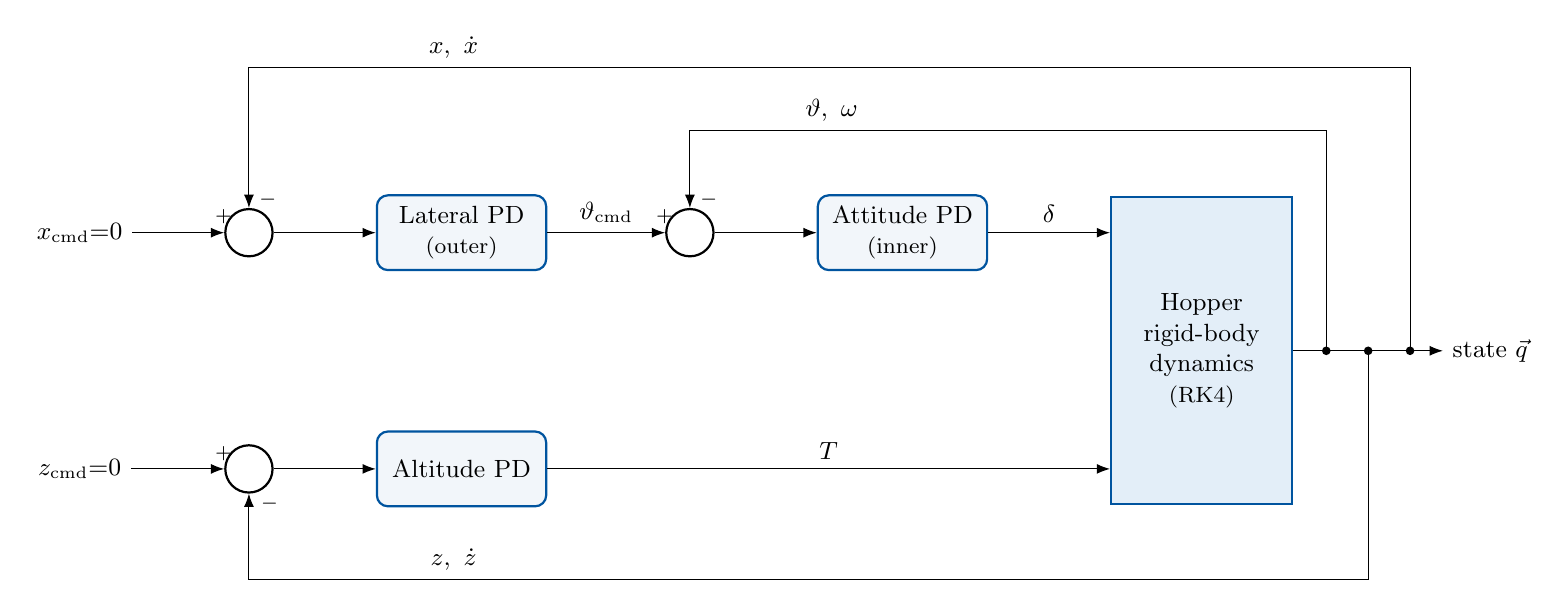
\begin{tikzpicture}[>=Latex, font=\small,
  sum/.style={draw, circle, minimum size=6mm, inner sep=0pt, thick},
  block/.style={draw=rwth, thick, rounded corners, align=center,
                minimum height=0.95cm, minimum width=2.15cm, fill=rwth!5},
  plant/.style={draw=rwth, thick, align=center, fill=rwthlight!25,
                minimum width=2.3cm, minimum height=3.9cm},
  dot/.style={circle, fill, inner sep=1.1pt}]

  \node[sum]   (s1)  at (0,0)      {};
  \node[block] (lat) at (2.7,0)    {Lateral PD\\\footnotesize(outer)};
  \node[sum]   (s2)  at (5.6,0)    {};
  \node[block] (att) at (8.3,0)    {Attitude PD\\\footnotesize(inner)};
  \node[plant] (plant) at (12.1,-1.5) {Hopper\\rigid-body\\dynamics\\\footnotesize(RK4)};

  \node[sum]   (s3)  at (0,-3)     {};
  \node[block] (alt) at (2.7,-3)   {Altitude PD};

  \node (xref) at (-2.15,0)  {$x_{\mathrm{cmd}}{=}0$};
  \node (zref) at (-2.15,-3) {$z_{\mathrm{cmd}}{=}0$};

  \draw[->] (xref) -- (s1);
  \draw[->] (s1) -- (lat);
  \draw[->] (lat) -- node[above] {$\vartheta_{\mathrm{cmd}}$} (s2);
  \draw[->] (s2) -- (att);
  \draw[->] (att) -- node[above] {$\delta$} (plant.west|-att);

  \draw[->] (zref) -- (s3);
  \draw[->] (s3) -- (alt);
  \draw[->] (alt) -- node[above] {$T$} (plant.west|-alt);

  \draw[->] (plant.east) -- ++(1.9,0)
        node[right] {state $\vec q$}
        coordinate[pos=0.22] (tapI)
        coordinate[pos=0.5]  (tapA)
        coordinate[pos=0.78] (tapO);
  \node[dot] at (tapI) {}; \node[dot] at (tapA) {}; \node[dot] at (tapO) {};

  \draw[->] (tapI) -- ++(0,2.8) -| (s2.north);
  \draw[->] (tapO) -- ++(0,3.6) -| (s1.north);
  \draw[->] (tapA) -- ++(0,-2.9) -| (s3.south);

  \node at (7.4,1.55)  {$\vartheta,\ \omega$};
  \node at (2.6,2.35)  {$x,\ \dot x$};
  \node at (2.6,-4.15) {$z,\ \dot z$};

  \node at (-0.32,0.20)  {\scriptsize$+$};  \node at (0.24,0.42)   {\scriptsize$-$};
  \node at (5.28,0.20)   {\scriptsize$+$};  \node at (5.84,0.42)   {\scriptsize$-$};
  \node at (-0.32,-2.80) {\scriptsize$+$};  \node at (0.26,-3.44)  {\scriptsize$-$};
\end{tikzpicture}%
}
\caption{The cascaded controller. The outer lateral loop commands a tilt $\vartheta_{\mathrm{cmd}}$ that the fast inner attitude loop follows through $\delta$; the altitude loop sets $T$ on its own. Each summing junction subtracts the fed-back state from the reference.}
\label{fig:cascade}
\end{figure}

\textbf{Each loop is a second-order system.} Close to vertical and near hover, each channel is just a double integrator driven by its input. In the altitude loop, if I cancel gravity with a feed-forward term, $T=mg+u_z$, then PD feedback $u_z=-K_p z-K_d\dot z$ gives
\begin{equation}
  \ddot z + 2\zeta\omega_n\,\dot z + \omega_n^2\,z = 0,
  \qquad \omega_n^2 = \frac{K_p}{m}, \qquad 2\zeta\omega_n = \frac{K_d}{m},
\end{equation}
The lateral and attitude loops look the same, except the $m$ in front is replaced by $m/T$ and $I/(\ell T)$. Since those depend on the current thrust, I schedule the lateral and attitude gains on $T$ to keep $\omega_n$ and $\zeta$ constant; the altitude loop just uses fixed gains.

\textbf{Why PD.} With $K_d=0$ each loop is just $\ddot z+\omega_n^2 z=0$, an undamped oscillator, so the lander would keep oscillating and never settle. The derivative term $2\zeta\omega_n\dot z$ damps that out, so PD is the simplest thing that works. I do not add an integral term because there is no steady disturbance or bias to cancel in this model; that would change with something like crosswinds or a mass/gravity mismatch. I pick the damping per loop. The altitude loop is critically damped ($\zeta=1$), since even one overshoot could put it into the ground on the way down. The lateral and attitude loops use $\zeta=0.7$, where a small overshoot is fine and the faster response matters, because the offset has to be gone before touchdown.

\begin{table}[H] \centering\small
\begin{tabular}{lllccl}
\hline
Loop & States & Output & $\omega_n$ (rad/s) & $\zeta$ & Limits\\
\hline
Altitude        & $z,\dot z$         & thrust $T$                          & 0.5 & 1.0 & $T \ge 0$\\
Lateral (outer) & $x,\dot x$         & tilt cmd $\vartheta_{\mathrm{cmd}}$ & 0.5 & 0.7 & $\pm 20^\circ$\\
Attitude (inner)& $\vartheta,\omega$ & gimbal $\delta$                     & 2.5 & 0.7 & $\pm 10^\circ$\\
\hline
\end{tabular}
\caption{The three PD loops. The inner loop is five times faster than the outer, so they can be tuned independently.}
\end{table}

\textbf{Saturation and cutoff.} The commanded tilt is limited to $\pm 20^\circ$ and the gimbal to $\pm 10^\circ$. The engine is cut below $0.10~\mathrm{m}$, so in the ideal case touchdown is a short free fall at $\sqrt{2g\cdot 0.1~\mathrm{m}}\approx0.57~\mathrm{m/s}$.

\section*{Two representative descents}
\textbf{Working case} (Figure~\ref{fig:work}; $x_0=2~\mathrm{m}$, $\vartheta_0=5^\circ$). The thrust stays at zero at first: the lander starts above the target altitude, so the altitude loop would want downward thrust, which clips to zero, and gravity does the early descent for free. The attitude stays constant while there is no thrust, since you cannot tilt without it. Once the thrust comes up, the gimbal tilts the body to cancel the sideways offset and only straightens it out once the offset is gone, so the lander ends up upright last; the sideways position overshoots a bit in the middle, as expected. Just before $13.5~\mathrm{s}$ it crosses the $0.10~\mathrm{m}$ cutoff and the engine shuts off. There is no overshoot in $z$.

\textbf{Failing case} (Figure~\ref{fig:fail}; $x_0=20~\mathrm{m}$, twice the initial height). The commanded tilt saturates at $-20^\circ$ to try to recover the large offset. The controller does bring $x$ back toward zero, but the recovery takes longer than the descent, so the lander is still leaning at touchdown ($\vartheta=+20^\circ$) with $v_x=-2.5~\mathrm{m/s}$: a crash. What matters here is how big an offset can be fixed in the time left before landing, not how big the initial tilt is.

\begin{figure}[H]
\centering
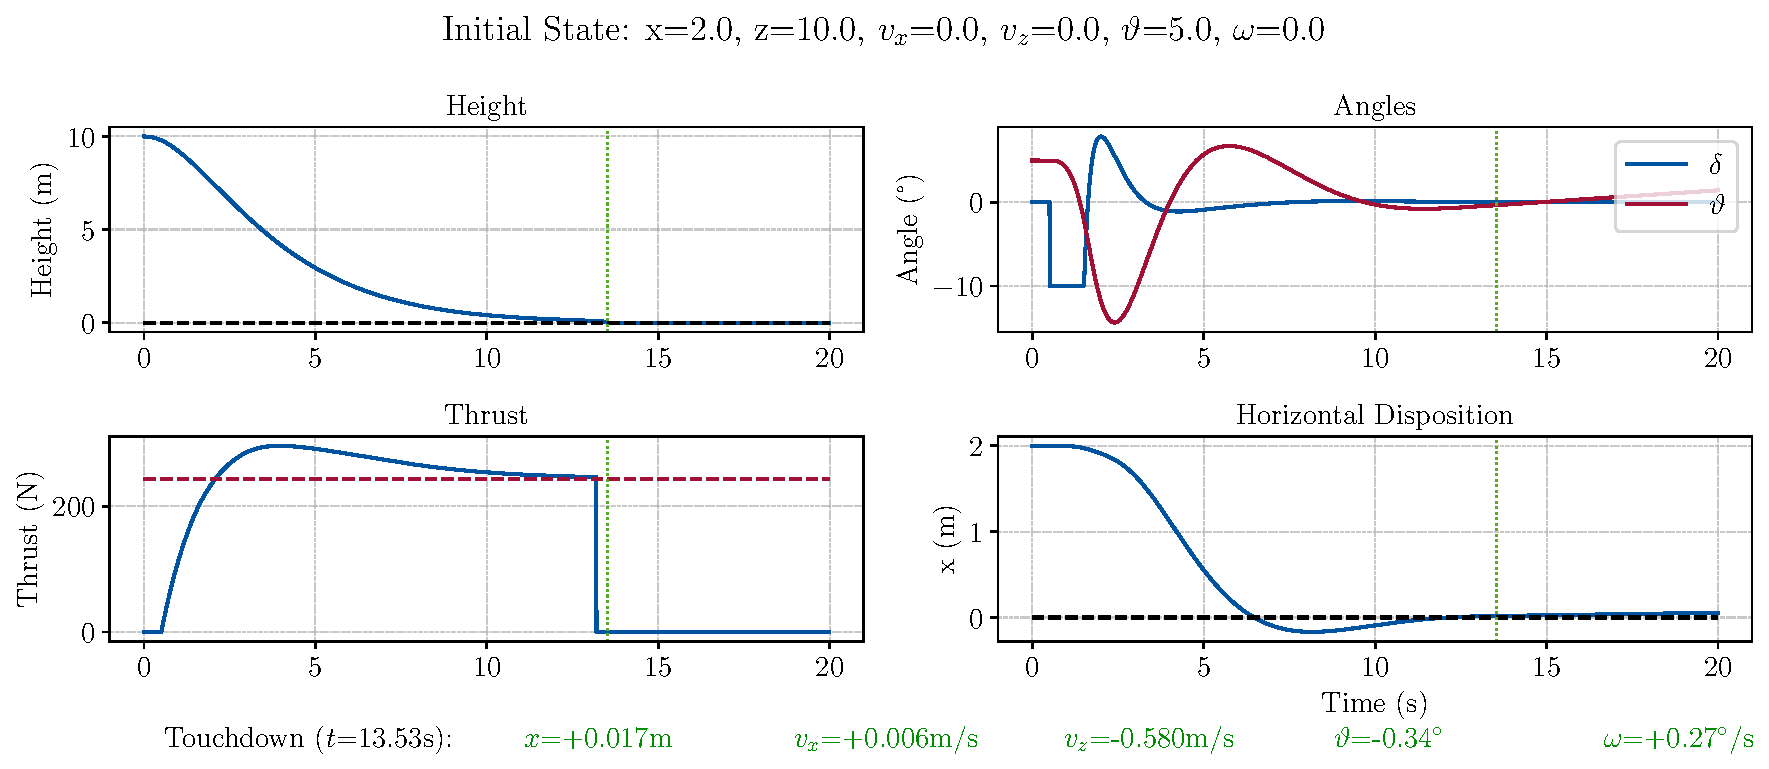
\includegraphics[width=0.93\linewidth]{Plots/hopper_work.pdf}
\caption{\textbf{Working case} ($x_0=2~\mathrm{m}$, $\vartheta_0=5^\circ$). Touchdown at $t=13.5~\mathrm{s}$: $x=+0.02~\mathrm{m}$, $v_x=+0.01~\mathrm{m/s}$, $v_z=-0.58~\mathrm{m/s}$, $\vartheta=-0.3^\circ$, a soft landing. The dotted green line marks touchdown; plots are truncated there.}
\label{fig:work}
\end{figure}

\begin{figure}[H]
\centering
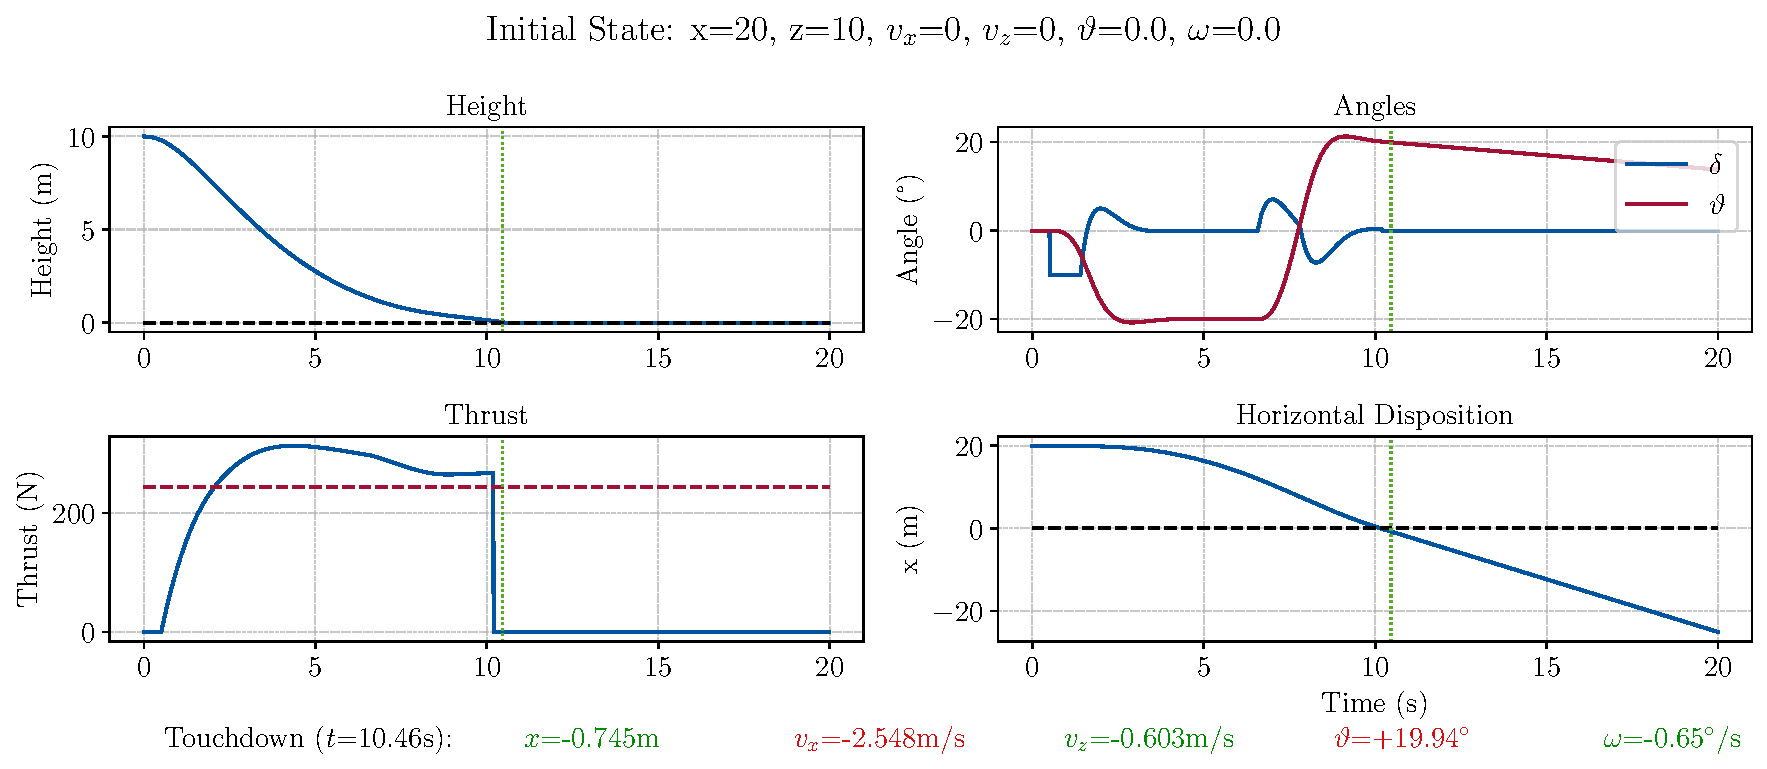
\includegraphics[width=0.93\linewidth]{Plots/hopper_fail.pdf}
\caption{\textbf{Failing case} ($x_0=20~\mathrm{m}$). The commanded tilt saturates at $-20^\circ$ to recover the offset; touchdown at $t=10.5~\mathrm{s}$ with $v_x=-2.5~\mathrm{m/s}$ and $\vartheta=+20^\circ$, a crash. The lateral-recovery manoeuvre outlasts the descent.}
\label{fig:fail}
\end{figure}

\section*{Monte Carlo dispersion analysis}
To test the controller more broadly, I run $N=1000$ descents with the initial conditions picked uniformly from $x_0\in[-5,5]~\mathrm{m}$, $\dot x_0\in[-2,2]~\mathrm{m/s}$, $\dot z_0\in[-3,0]~\mathrm{m/s}$, $\vartheta_0\in[-10^\circ,10^\circ]$, $\omega_0\in[-3^\circ,3^\circ]/\mathrm{s}$, all from $z_0=10~\mathrm{m}$. I call a landing \emph{soft} if $|x|<0.5~\mathrm{m}$, $|v_x|<0.5~\mathrm{m/s}$, $|v_z|<1~\mathrm{m/s}$, $|\vartheta|<5^\circ$, and \emph{acceptable} if it meets the looser limits $|x|<1~\mathrm{m}$, $|v_x|<1~\mathrm{m/s}$, $|v_z|<2~\mathrm{m/s}$, $|\vartheta|<10^\circ$ but is not soft.

Flying on the true state, \textbf{830 (83.0\,\%) were soft} and 52 acceptable, so \textbf{882 (88.2\,\%) within tolerance} and \textbf{118 (11.8\,\%) failures}, all of them out-of-tolerance touchdowns, no timeouts. The touchdown scatter (Figure~\ref{fig:mc}, right) shows the sideways velocities staying inside $|v_x|<1~\mathrm{m/s}$, while the failures all have touchdown tilt above $10^\circ$. That tilt does not come from large initial tilts (those correct quickly), it comes from large initial sideways offsets: to cancel an offset the lander has to hold a tilt, and that tilt is not always straightened out in time.

\begin{figure}[H]
\centering
\begin{minipage}{0.49\linewidth}\centering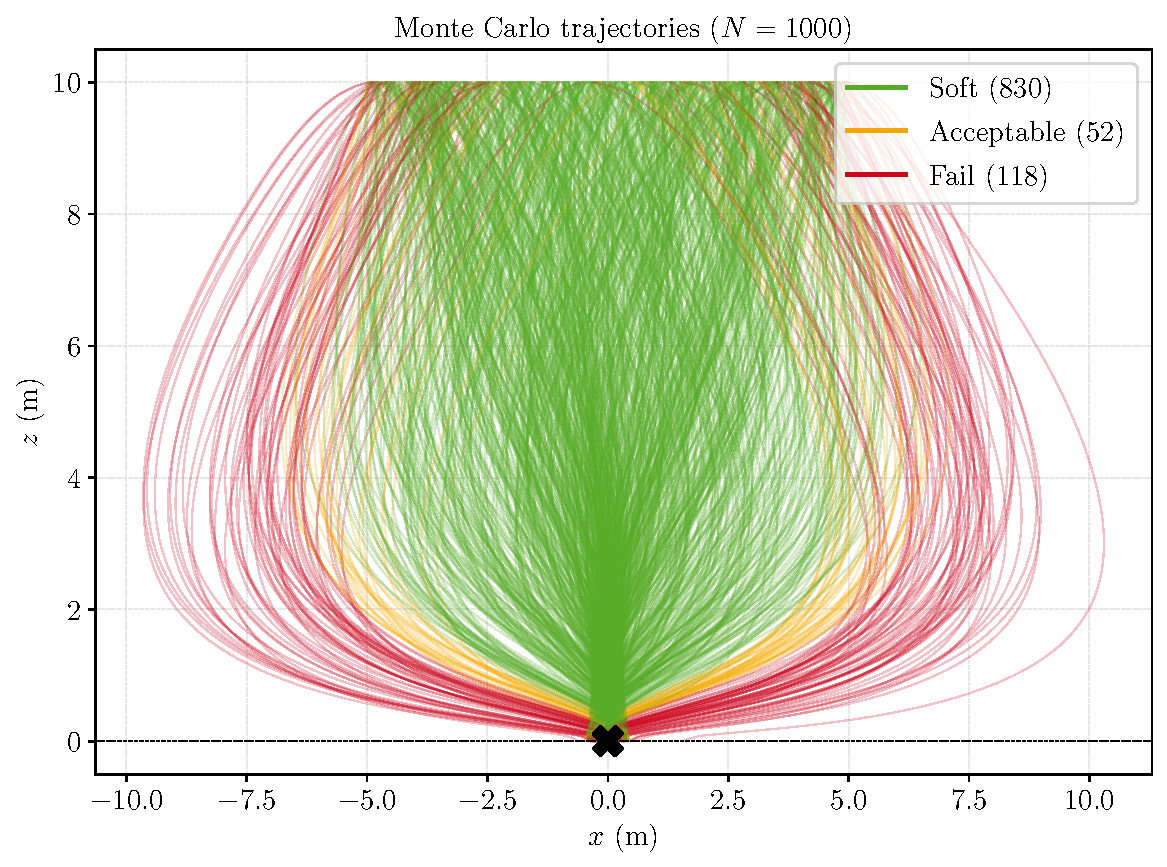
\includegraphics[width=\linewidth]{Plots/mc_trajectories.pdf}\end{minipage}\hfill
\begin{minipage}{0.49\linewidth}\centering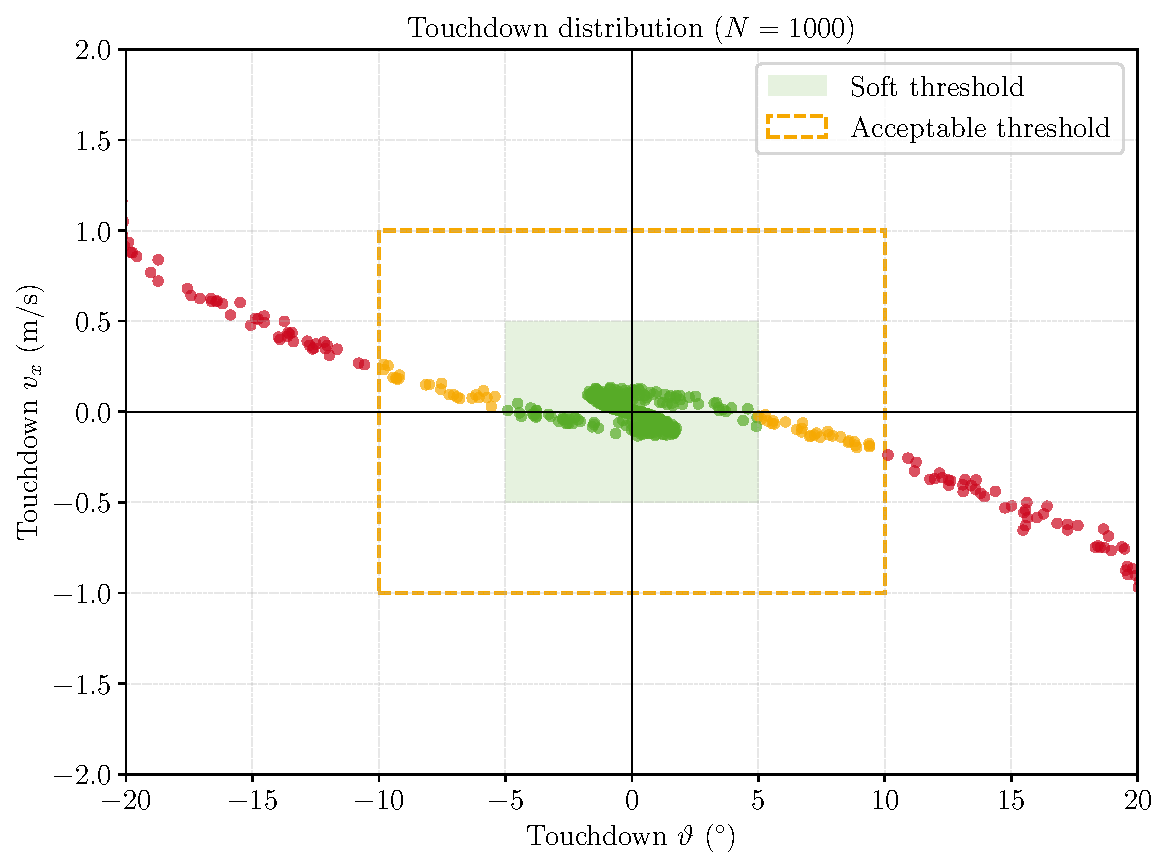
\includegraphics[width=\linewidth]{Plots/mc_touchdown.pdf}\end{minipage}
\caption{Monte Carlo, perfect state ($N=1000$). \textbf{Left:} trajectories coloured by outcome. \textbf{Right:} touchdown distribution in the $\vartheta$--$v_x$ plane against the soft (shaded) and acceptable (dashed) limits; marker colour reflects the classification.}
\label{fig:mc}
\end{figure}

\section*{Navigation: flying on an estimate}
So far the controller gets the true state, which a real vehicle does not have. The navigation layer adds sensors and an Extended Kalman Filter that estimates the four translational states $s=(x,z,\dot x,\dot z)$; attitude is still taken as known. I model two sensors: an accelerometer read every step, which measures the specific force (the thrust acceleration, not gravity) plus white noise, and an altimeter read once every $0.2~\mathrm{s}$, which measures altitude plus white noise.

The filter keeps a Gaussian estimate of $s$ (a mean and a covariance) and updates it in two steps. The \emph{predict} step dead-reckons on the accelerometer: it moves the mean forward with the measured acceleration and grows the covariance to account for the noisy reading and the imperfect model. The \emph{update} step runs only when an altimeter reading comes in: it compares the altitude the filter expected with what the altimeter actually read, and moves the mean toward the reading, with how much depending on which one it trusts more, while shrinking the covariance. Two things matter here. With attitude known, both the dynamics and the measurement are linear in $s$, so the EKF is really just a linear Kalman filter. And the altimeter only sees altitude, so horizontal position is never measured directly: it is dead-reckoned and drifts with any error in the initial velocity, which ends up being the main source of error.

\textbf{Results.} Running the same 1000 runs on the estimate instead of the truth (Table~\ref{tab:compare}, Figure~\ref{fig:ekf}), the \textbf{soft rate drops from $83.0\%$ to $58.6\%$}, while the \textbf{within-tolerance rate barely changes, $88.2\%$ to $84.0\%$}. The reason is what the sensors can see. The altimeter holds the vertical channel, so the descent and the cutoff timing stay about the same and few landings drop out of tolerance. Horizontal position is not measured, so it drifts, and that drift pushes tight soft landings into the wider acceptable band. The estimate-versus-truth plots show this: $z$, $\dot x$ and $\dot z$ track well, and only $x$ keeps a small bias that no sensor can remove. To check the filter is consistent, I run it over 300 random descents: the 4-state NEES sits at $4.0$ and the altimeter NIS at $1.0$, both inside their 95\,\% bands, so the covariance it reports matches its real error. The lost soft landings are not a tuning issue, they are the price of never measuring horizontal position.

\begin{table}[H]\centering\small
\begin{tabular}{lcc}
\hline
Outcome & Perfect state & EKF estimate\\
\hline
Soft                                   & 83.0\,\% & 58.6\,\%\\
Within tolerance (soft or acceptable)  & 88.2\,\% & 84.0\,\%\\
Failure                                & 11.8\,\% & 16.0\,\%\\
\hline
\end{tabular}
\caption{Landing outcomes over the same $N=1000$ runs, controller flown on truth versus on the EKF estimate.}
\label{tab:compare}
\end{table}

\begin{figure}[H]
\centering
\begin{minipage}{0.72\linewidth}\centering
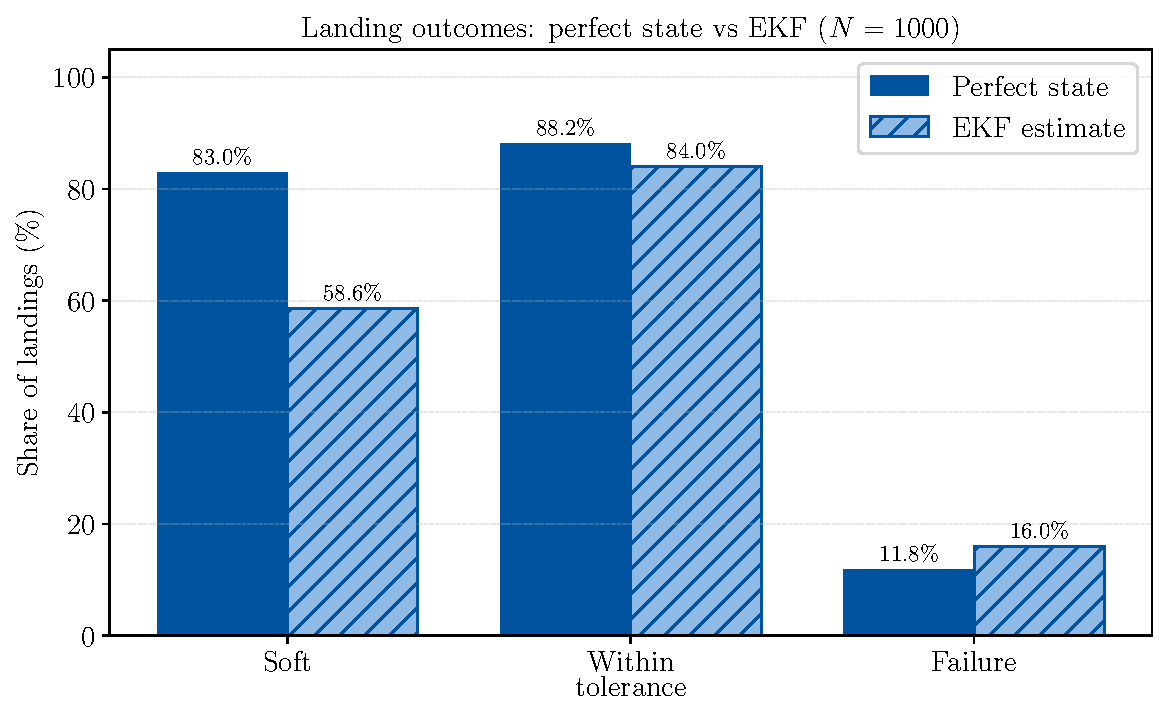
\includegraphics[width=\linewidth]{Plots/mc_perfect_vs_ekf.pdf}
\end{minipage}
\begin{minipage}{\linewidth}\centering
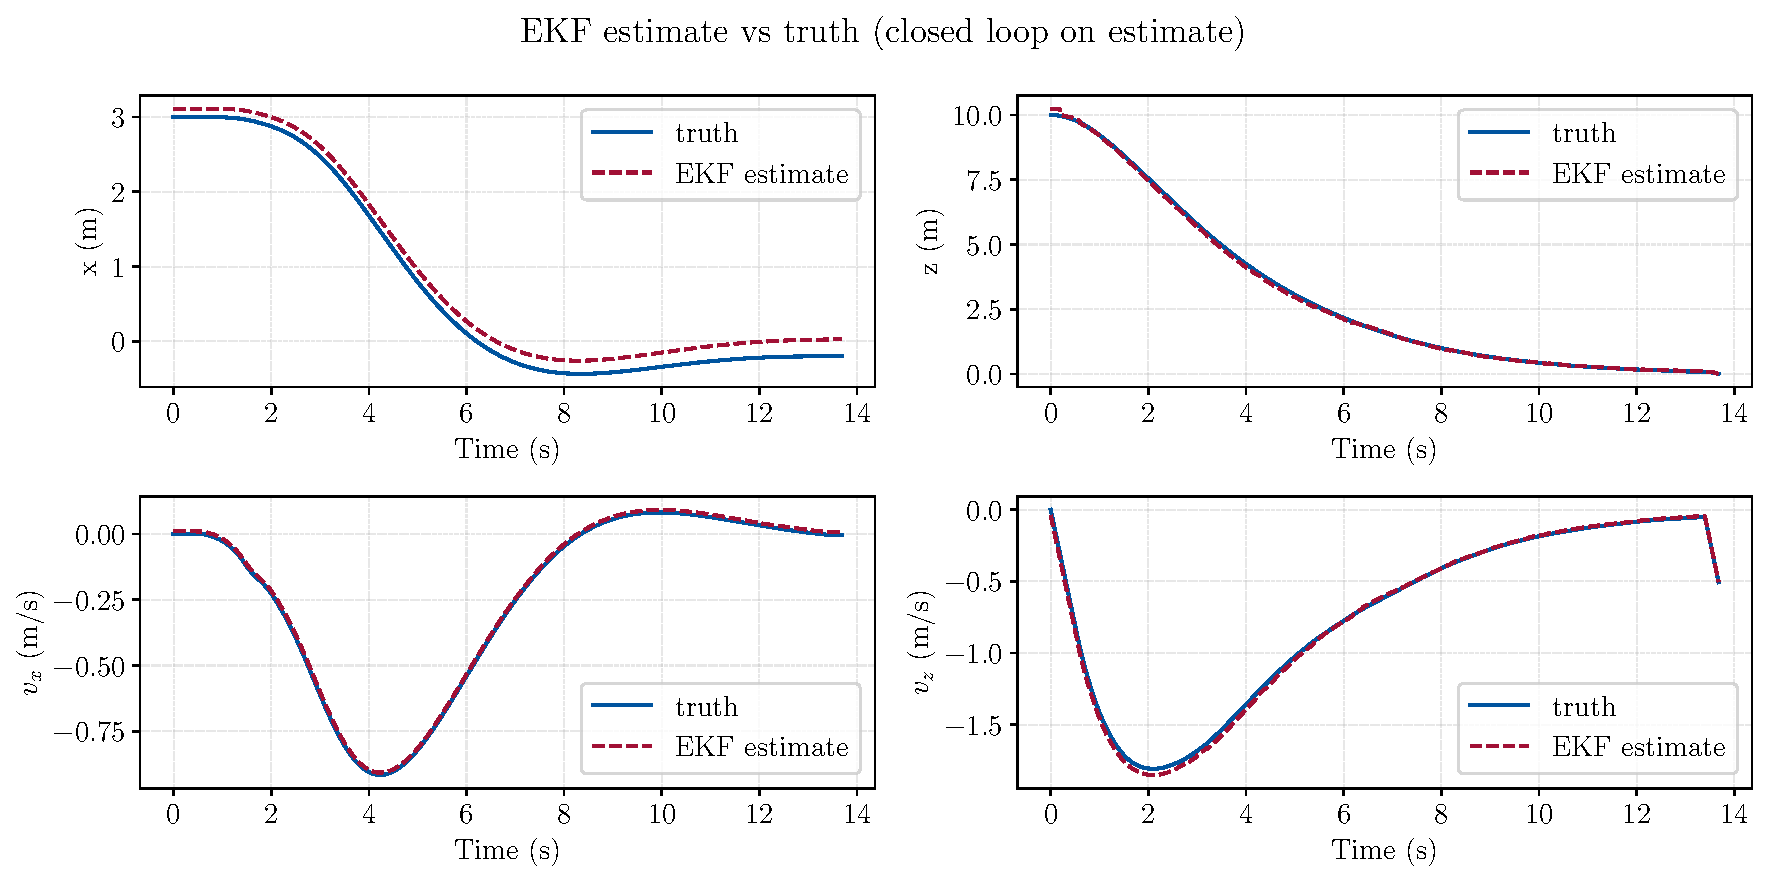
\includegraphics[width=\linewidth]{Plots/ekf_estimate_vs_truth.pdf}
\end{minipage}
\caption{\textbf{Top:} outcome shares, perfect state (solid) versus EKF estimate (hatched); the loss is soft landings shifting into the acceptable band. \textbf{Bottom:} estimate versus truth on one descent. Only $x$ carries a lasting bias, since horizontal position is never measured.}
\label{fig:ekf}
\end{figure}

\section*{Limitations and outlook}
The lander is reactive: it corrects errors as they appear, with no trajectory planning or fuel optimisation, and it relies on the offsets being correctable before touchdown. Its limits point straight at the methods it does not use. The next step would be optimisation-based guidance, where fuel, actuator and state limits enter as explicit constraints, so the large-offset regime is handled by planning the trajectory instead of reacting to it, and the touchdown limits are met by construction rather than checked afterwards. On the navigation side, the one real gap is horizontal position: a terrain-relative or Doppler velocity sensor would measure the channel the altimeter cannot. Going from reactive robustness towards designed-in robustness is the direction I would like to take this.

\vspace{2pt}
{\footnotesize\itshape Implemented in Python (NumPy): RK4 propagator, cascaded gain-scheduled PD controller, Extended/linear Kalman Filter, Monte Carlo campaign, all seeded and reproducible. Full code at \url{https://github.com/Krautsalat13/LunarHopper}.}
\end{document}
